%%%%%%%%%%%%%%%%%%%%%%%%%%%%%%%%%%%%%%%%%
% Dreuw & Deselaer's Poster
% LaTeX Template
% Version 1.0 (11/04/13)
%
% Created by:
% Philippe Dreuw and Thomas Deselaers
% http://www-i6.informatik.rwth-aachen.de/~dreuw/latexbeamerposter.php
%
% This template has been downloaded from:
% http://www.LaTeXTemplates.com
%
% License:
% CC BY-NC-SA 3.0 (http://creativecommons.org/licenses/by-nc-sa/3.0/)
%
%%%%%%%%%%%%%%%%%%%%%%%%%%%%%%%%%%%%%%%%%

%----------------------------------------------------------------------------------------
%	PACKAGES AND OTHER DOCUMENT CONFIGURATIONS
%----------------------------------------------------------------------------------------

\documentclass[final,hyperref={pdfpagelabels=false}]{beamer}

\usepackage[orientation=portrait,size=a0,scale=1.4]{beamerposter} % Use the beamerposter package for laying out the poster with a portrait orientation and an a0 paper size

\usetheme{I6pd2} % Use the I6pd2 theme supplied with this template

\usepackage[english]{babel} % English language/hyphenation
\usepackage[utf8]{inputenc} % Required for inputting international characters
%\usepackage[T1]{fontenc}
\usepackage{algorithm}
\usepackage[noend]{algpseudocode}
\usepackage{hyperref}

\usepackage{amsmath,amsthm,amssymb,latexsym} % For including math equations, theorems, symbols, etc

%\usepackage{times}\usefonttheme{professionalfonts}  % Uncomment to use Times as the main font
%\usefonttheme[onlymath]{serif} % Uncomment to use a Serif font within math environments

\boldmath % Use bold for everything within the math environment

\usepackage{booktabs} % Top and bottom rules for tables

\graphicspath{{figures/}} % Location of the graphics files

\usecaptiontemplate{\small\structure{\insertcaptionname~\insertcaptionnumber: }\insertcaption} % A fix for figure numbering

%----------------------------------------------------------------------------------------
%	TITLE SECTION 
%----------------------------------------------------------------------------------------

\title{\huge Teoria dos Números e Computação: \\ \normalsize Uma abordagem utilizando problemas de competições de programação} % Poster title
\bigskip

\author{Autor: Antonio Roberto de Campos Junior \\ Supervisor: Carlos Eduardo Ferreira} % Author(s)

\institute{Instituto de Matemática e Estatística - Universidade de São Paulo} % Institution(s)

%----------------------------------------------------------------------------------------
%	FOOTER TEXT
%----------------------------------------------------------------------------------------

\newcommand{\leftfoot}{http://www.ime.usp.br} % Left footer text

\newcommand{\rightfoot}{robertojr.bcc@gmail.com} % Right footer text

%----------------------------------------------------------------------------------------

\begin{document}

\addtobeamertemplate{block end}{}{\vspace*{2ex}} % White space under blocks

\begin{frame}[t] % The whole poster is enclosed in one beamer frame

\begin{columns}[t] % The whole poster consists of two major columns, each of which can be subdivided further with another \begin{columns} block - the [t] argument aligns each column's content to the top

\begin{column}{.02\textwidth}\end{column} % Empty spacer column

\begin{column}{.465\textwidth} % The first column

%----------------------------------------------------------------------------------------
%	OBJECTIVES
%----------------------------------------------------------------------------------------

\begin{block}{Objetivos}

\begin{enumerate}
\item Estudar tópicos específicos relacionados à Teoria dos Números;
\item Criar um material que mostre a aplicação direta dessa teoria na solução de problemas de competições de programação;
\item Demonstração da teoria e implementação dos algoritmos que resolvem os problemas que serão abordados;
\end{enumerate}

\end{block}

%----------------------------------------------------------------------------------------
%	INTRODUCTION
%----------------------------------------------------------------------------------------
            
\begin{block}{Introdução}

\begin{itemize}
\item Teoria do Números é um vasto ramo da matemática que estuda números inteiros. Números primos, fatorização de números inteiros, funções aritméticas, são alguns dos tópicos mais estudados e também importantes para resolução de problemas computacionais.

Hoje em dia a importância da Teoria do Números na Computação é inquestionável, e desse modo, esse trabalho vem ilustrar como a teoria pode ser aplicada na criação de algoritmos para resolução de problemas computacionais, em especial problemas de competições de programação.

Equações diofantinas, Congruência Modular, Números de Fibonacci, são alguns dos assuntos que serão abordados nesse trabalho. Após a devida demostração da teoria serão exibidos alguns problemas de competições de programação que aplicam essa teoria, seguido da implementação e análise do algoritmo que resolve o problema abordado.
\end{itemize}

\end{block}

%----------------------------------------------------------------------------------------
%	Problema
%----------------------------------------------------------------------------------------

\begin{block}{Problema exemplo: Skyscraper Floor}

\textbf{Resumo do problema: }
É dado um prédio com $F$ andares (numerados de $0$ até $F-1$) e $E$ elevadores. Cada elevador $i$ tem um posição inicial $Y_i$ ($Y_i \geq 0$) e uma constante $X_i$ ($X_i > 0$),
de tal forma que os únicos andares que esse elevador consegue chegar são da forma, $Y_i+X_it$, com $t$ inteiro.
Cada elevador $i$ não consegue atingir andares menores que $Y_i$ e maiores ou iguais à $F$, ie, $Y_i \leq Y_i+X_it \leq F-1$, ou melhor, $0 \leq t \leq \frac{F-1-Y_i}{X_i}$.
Dado os valores $F$, $E$, e as constantes $Y_i$, $X_i$ para cada elevador, o problema consite em verificar se é possível ir do andar $A$ até o andar $B$ ($0\leq A,B <F$)
usando os $E$ elevadores.


\end{block}

%----------------------------------------------------------------------------------------
%	METHODS
%----------------------------------------------------------------------------------------

\begin{block}{Solução Parte 1}

\textbf{Proposição 1: }
Tome $[d,x_0,y_0]$ como sendo a tupla retornada pelo $ExtendedMDC(a,b)$, com $a$, $b$, $c$ inteiros e $MDC(a,b)|c$.
Então temos que todas as soluções da equação $ax+by=c$ são da forma: $x=(x_0\frac{c}{d} + \frac{bq}{d})$, $y=(y_0\frac{c}{d} - \frac{aq}{d})$, em que $q\in\mathbb{Z}$.

\textbf{Teorema 1: }
Dados inteiros $a$, $b$, $c$ , temos que:
$MDC(a,b)|c \Leftrightarrow$ a \textit{Equação Diofantina} $ax + by=c$, tem solução inteira.

\textbf{Obs.:} A proposição e o teorema citados acima foram devidamente demonstrados na monografia correspondente a esse poster encontrada em: \href{https://github.com/AntonioRoberto/monografia/blob/master/main.pdf}{https://github.com/AntonioRoberto/monografia/blob/master/main.pdf}.
\newline

\textbf{Solução: }Primeiro imagine que temos um grafo bidirecionado com $E$ vértices, onde cada vértice representa um elevador e cada aresta $(u,v)$ nos diz que os elevadores $u$ e $v$
conseguem chegar em algum andar em comum.
Sabemos quais elevadores atingem o andar $A$, basta verificar se $Y_i+X_it=A$ tem solução $t$ inteira. Analogamente sabemos quais elevadores atingem o andar
$B$. Então só precisaríamos fazer uma busca (\href{https://en.wikipedia.org/wiki/Breadth-first_search}{BFS} ou \href{https://en.wikipedia.org/wiki/Depth-first_search}{DFS})
nesse grafo e verificar se há um caminho de um elevador que atinge o andar $A$ até algum elevador que atinge o andar $B$.

Porém, para esse problema, não entraremos em detalhe nos algoritmos envolvendo grafos. Nos focaremos na parte matemática do problema, que envolve descobrir quando dois elevadores conseguem chegar em algum andar em comum, nos possibilitando assim, construir o grafo e resolver o problema.

Dois elevadores $u$ e $v$ tem um andar em comum, se existe inteiros $t_u$ ($0\leq t_u\leq \frac{F-1-Y_u}{X_u}$) e $t_v$ ($0\leq t_v\leq \frac{F-1-Y_v}{X_v}$), tal que
$Y_u+X_ut_u = Y_v+X_vt_v$, o que nos dá a \textit{Equação Diofantina Linear} $X_ut_u + (-X_v)tv = (Y_v-Y_u)$.



\end{block}
%----------------------------------------------------------------------------------------

\end{column} % End of the first column

\begin{column}{.03\textwidth}\end{column} % Empty spacer column
 
\begin{column}{.465\textwidth} % The second column
%----------------------------------------------------------------------------------------
\begin{block}{Solução Parte 2}


Vamos mostrar agora um método para calcular $t_u$ e $t_v$, tal que $at_u + bt_v = c$, com $a=X_u$, $b=-X_v$ e c=$(Y_v-Y_u)$.
Pelo \textbf{Teorema 1}, sabemos que essa equação tem solução, se e somente se, $MDC(a,b)|c$. Observe também que se $Y_u=Y_v$ os elevadores estarão
conexos pelo andar $Y_u$. Checaremos essas restrições no começo do algoritmo, e daqui para frente assumiremos que $MDC(a,b)|c$ e $Y_u\neq Y_v$.

Tome $t_1$, $t_2$ como sendo uma solução qualquer da equação diofantina $at_1+bt_2 = MDC(a,b)=d$ (Observe que $t_1$ e $t_2$ podem ser calculados com o \textit{Algoritmo Extendido de Euclides}), temos então pelo \textbf{Proposição 1} que todas as soluções da
equação $at_u + bt_v = c$, são da forma $t_u = (t_1\frac{c}{d} + \frac{bq}{d})$ e $t_v = (t_2\frac{c}{d} - \frac{aq}{d})$, com $q \in\mathbb{Z}$. Logo:
\\

$t_u = (t_1\frac{c}{d} + \frac{bq}{d}) \Rightarrow \frac{-t_1c}{b} \leq q \leq \big[(\frac{F-1-Y_u}{X_u})d - t_1c\big]\frac{1}{b}$, já que $0\leq t_u\leq \frac{F-1-Y_u}{X_u}$
\\

Analogamente temos:
\\

$t_v = (t_2\frac{c}{d} - \frac{aq}{d}) \Rightarrow \frac{t_2c}{a} \geq q \geq \big[t_2c - (\frac{F-1-Y_v}{X_v})d\big]\frac{1}{a}$, já que $0\leq t_u\leq \frac{F-1-Y_u}{X_u}$
\\

Das duas inequações acima, temos:
\\

$max\Big(\frac{-t_1c}{b}, \big[t_2c - (\frac{F-1-Y_v}{X_v})d\big]\frac{1}{a} \Big) \leq q \leq min\Big(\frac{t_2c}{a}, \big[(\frac{F-1-Y_u}{X_u})d - t_1c\big]\frac{1}{b}  \Big)$
\\

Portanto, se a inequação acima tiver solução inteira $q$, os elevadores $u$ e $v$ serão conectados pelo andar $Y_u+X_ut_u = Y_u+X_u\big[(t_1 + \frac{bq}{d})\frac{c}{d}\big]$.
\\
\end{block}



%----------------------------------------------------------------------------------------
% Codigo
%----------------------------------------------------------------------------------------

     
%----------------------------------------------------------------------------------------
%Curiosidades
%----------------------------------------------------------------------------------------

\begin{block}{Curiosidades da ACM-ICPC}

ACM-ICPC (International Collegiate Programming Contest) é uma competição de programação
de várias etapas e baseada em equipe. O principal objetivo é encontrar algoritmos
eficientes, que resolvem os problemas abordados pela competição, o mais rápido
possível.


Nos últimos anos a ACM-ICPC teve um crescimento significativo. Se compararmos
o número de competidores, temos que de 1997 (ano em que começou o patrocinio
da IBM) até 2014 houve um aumento maior que $1500\%$, totalizando 38160
competidores de 2534 universidades em 101 países ao redor do mundo.

Para mais informa\c{c}\~oes sobre as competi\c{c}\~oes passadas acesse \href{icpc.baylor.edu}{icpc.baylor.edu}.
\newline
\begin{figure}%[!htb]
    %\centering
    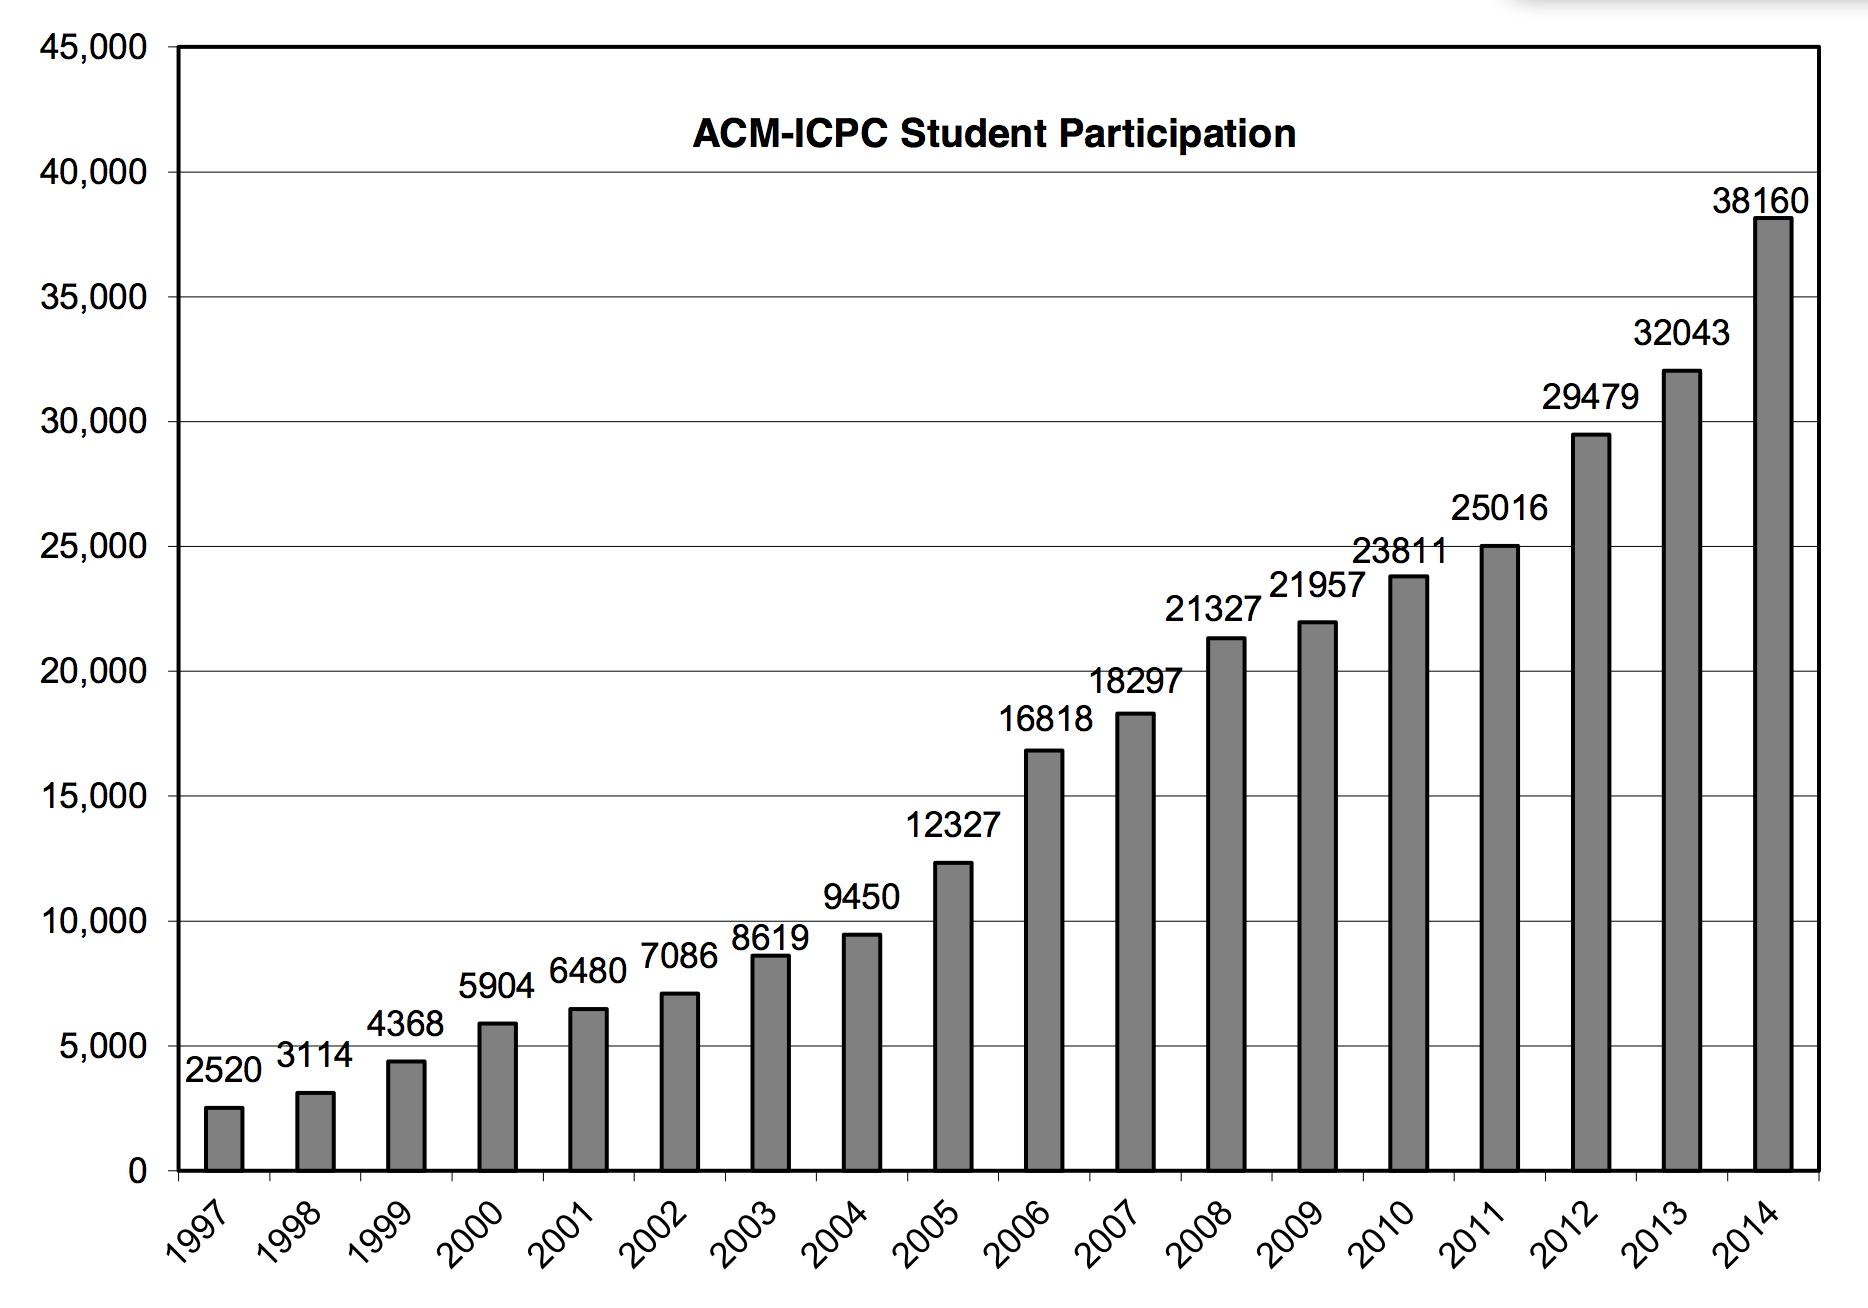
\includegraphics[width=0.8\linewidth]{grafico.png}
    \caption{Crescimento do n\'umero de participantes por ano.}
\end{figure}



\end{block}


%----------------------------------------------------------------------------------------
%	ACKNOWLEDGEMENTS
%----------------------------------------------------------------------------------------

\begin{block}{Acknowledgments}

\begin{itemize}
\item Carlos Eduardo Ferreira - Auxílio durante todo o desenvolvimento desse trabalho
\item Renzo Gomez Dias - Revisão dos textos
\end{itemize}

\end{block}

%----------------------------------------------------------------------------------------
%	CONTACT INFORMATION
%----------------------------------------------------------------------------------------

\setbeamercolor{block title}{fg=black,bg=orange!70} % Change the block title color

\begin{block}{Informações para Contato}

\begin{itemize}
\item Web: \href{http://www.ime.usp.br/~arcjr}{http://www.ime.usp.br/~arcjr}
\item Email: \href{mailto:john@smith.com}{robertojr.bcc@gmail.com}
\end{itemize}

\end{block}

%----------------------------------------------------------------------------------------

\end{column} % End of the second column

\begin{column}{.015\textwidth}\end{column} % Empty spacer column

\end{columns} % End of all the columns in the poster

\end{frame} % End of the enclosing frame

\end{document}
